
\documentclass[12pt]{article}
\usepackage{fullpage,amsmath,amssymb,graphicx}

\usepackage{setspace}
\spacing{1}

\usepackage{textpos}
\usepackage{tikz}
\usepackage{pgf}
\usepackage{amssymb}
\usepackage{enumerate}
\usepackage{xcolor}
\usepackage{graphicx}
\usepackage{subcaption}
\usepackage{tabularx}
\usepackage{colortbl}
\usepackage{multicol}
\usepackage{longtable}
\usepackage{hyperref}
\usepackage{comment}
\usepackage{listings}



\definecolor{encabezado}{rgb}{0.74, 0.83, 0.9}

\begin{document}

\hfill\\
\rule{\textwidth}{1.5pt}

\begin{minipage}[t]{85mm}
  \begin{tabular}{l}
    \textbf{\large Instituto Tecnológico de Costa Rica} \\  
    \textbf{Escuela de Ingeniería Electrónica} \\
    \textbf{Trabajo Final de Graduación} \\
    \textbf{Proyecto:} Método basado en aprendizaje reforzado \\para el control automático de una planta no lineal. \\
    \textbf{Estudiante:} Oscar Andrés Rojas Fonseca \hspace{3cm}\rule{4.5cm}{1.5pt}\\
    I Semestre 2024 \hspace{8.5cm}\textbf{Firma del asesor}
  \end{tabular}
\end{minipage}
\hfill\\
\rule{\textwidth}{1.5pt}


\section*{Bitácora de trabajo}

%\begin{table}[h]
\begin{minipage}[h]{\textwidth}
	\centering
	\begin{tabularx}{\textwidth}{|p{2cm}|X|X|p{2cm}|} 
		\hline
		\rowcolor{encabezado}
		\textbf{Fecha} & 
		\textbf{Actividad} & 
		\textbf{Anotaciones} & 
		\textbf{Horas dedicadas} \\ \hline
		% ***************************************************************
	 	01/04/2024 & 
	 	$\mathbf{1}.$ Continuación de revisión del código original para $DQN$ \cite{DQNCart}. & 
	 	$a)$ Identificación de la estructura del código ya facilitada ($Imports$, $Memory$, $DQN\,\, Algorithm$ y $Training$) y sub etapas (funciones importantes). \newline & 
	 	4 horas \\
		% ***************************************************************
		02/04/2024 & 
	 	$\mathbf{2}.$ Continuación de revisión del código original para $DQN$ \cite{DQNCart}. &
	 	$a)$ Estudio de las funciones de optimización ($optimize\_ model()$) y selección de acciones ($select\_ action()$). \newline & 
	 	2 horas \\
	 	% ***************************************************************
		02/04/2024 & 
	 	$\mathbf{3}.$ Prueba de implementación CUDA en env anaconda Ubuntu. &
	 	$a)$ Eliminación y replanteo de env conda con énfasis en herramientas $pytorch$ y CUDA. \newline
	 	$b)$ Resultado de la prueba: fallida, apunta a problemas de versiones. \newline & 
	 	6 horas \\
	 	% ***************************************************************
	 	03/04/2024 & 
	 	$\mathbf{4}.$ Reunión de seguimiento con el profesor asesor del proyecto. & 
	 	$a)$ Revisión de avance en el código y errores de forma.  \newline
	 	$b)$ Dado el factor tiempo y el poco avance realizado, se acordó enfocarse directamente en el env $Pendulum$ de Gymnasium \cite{gym}.  \newline & 
	 	2 horas \\
	 	\hline
	\end{tabularx}
\end{minipage}	 	
	 	
	 	% ***************************************************************
\hfill\\
\begin{minipage}[h]{\textwidth}
	\centering
	\begin{tabularx}{\textwidth}{|p{2cm}|X|X|p{2cm}|} 
		\hline		
		
	 	% ***************************************************************
	 	04/04/2024 & 
	 	$\mathbf{5}.$ Pruebas con entorno $CartPole$ y $Pendulum$ para implementación de CUDA. &
	 	$a)$ Por recomendación del profesor asesor, la implementación se mudó a Ubuntu/Linux para meyor control y referencia. \newline
	 	$b)$ Instalación y creación de nuevos $environments$ mediante la herramienta $micro\, mamba$. \newline & 
	 	6 horas \\
	 	% ***************************************************************
	 	05/04/2024 & 
	 	$\mathbf{6}.$ Estudio de las implicaciones de variación en el algoritmo $DQN$ \cite{DQNCart} de dos salidas discretas ($CartPole$) a una salida continua ($Pendulum$). &
	 	$a)$ Se identificaron los puntos clave a remplazar o modificar para el manejo de variables continuas. \newline
	 	$b)$ Las primeras pruebas de modificación apuntan a una necesidad de discretización del rango de torque ($[-2.0, \,\, 2.0]$) para adaptar el modelo al env $Pendulum$. \newline & 
	 	4 horas \\
	 	% ***************************************************************
	 	
	 	\hline
		\multicolumn{3}{|r|}{Total de horas de trabajo:} & 24 horas \\ 
	 	\hline                 
	\end{tabularx}
\end{minipage}
%\end{table}



% *****************************************************************************
% *****************************************************************************
% *****************************************************************************

\section*{Discusión}

\subsection*{Código referencia a método $DQN$ \cite{DQNCart}}

El código de implementación de control al env $CartPole$ de Gymnasium mediante $DQN$ presente mucho potencial para su adaptación al env $Pendulum$, en primera instancia y luego para experimentación previa al PAMH. Se encuentra debidamente comentado y su estructura esta clara y sencilla.

Luego de la reunión de seguimiento con el profesor asesor, se acordó saltar directamente a las pruebas con $Pendulum$ dados los problemas de tiempo del proyecto. Además, se detallaron puntos importantes al respecto como la diferenciación entre los tipos de $action space$ que presentan cada uno de los envs en cuestión, donde $CartPole$ implementa 
\[Discrete(2)\]
donde las dos posibles opciones son el $0$ para mover el carro base a la izquierda y $1$ para mover el carro base a la derecha.

Por otro lado, $Pendulum$ utiliza la estructura
\[Box(-2.0,\,\, 2.0,\,\, (1,),\,\, float32)\]
referente a un solo valor de acción posible de tipo decimal y en el rango permitido de $[-2.0,\,\, 2.0]$.

Lo anterior apunta a la necesidad de una manipulación superficial de la red neuronal base (capa de salida) y la función $select_action()$, función directamente asociada a la estructura de la red neuronal y puente para el $step()$ del env Gymnasium.


\subsection*{Errores de implementación $CUDA$ y $Pytorch$}

El código de referencia \cite{DQNCart} cuenta con la opción para utilizar CUDA con GPU y optimzar el tiempo de entrenamiento, con valores definidos claramente de $600$ episodios con GPU y $50$ episodios con CPU, donde ya el segundo demuestra la necesidad del uso de CUDA.

Sin embargo, las pruebas realizadas para su utilización arrojan varios errores referentes, en principio, a las versiones de todos los paquetes implicados; CUDA ($11.8$, $12.1$, $12.4$), $Pytorch$ ($2.1.2$, $2.2.2$) y el controlador de la GPU en Ubuntu (versión $535$). 

Todas las pruebas de env realizadas se evidencian con el comando
\[print(torch.cuda.is\_ available())\]
donde una respuesta de $False$ demuestra el problema de incongruencia entre versiones y en ocasiones tampoco se determina bien las razones del error. En proceso de resolución.

%\begin{figure}[h]
%	\centering
%	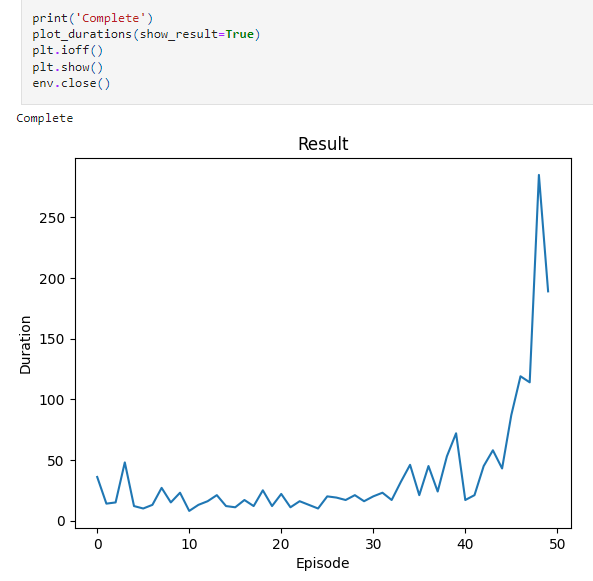
\includegraphics[scale=0.6]{Fig/CapturaCartPole1.png}
%	\caption{Resultado de entrenamiento del modelo para $CartPole$ con $50$ episodios.}
%	\label{fig:Cart1}
%\end{figure}	

\newpage

\section*{Referencias}
\renewcommand\refname{}
\bibliographystyle{IEEEtran}
\bibliography{references}





\end{document}
